\chapter{Asking Beverly Hills Billionaires How They Got Rich}

This chapter comes from a street lecture rather than a classroom lecture, but it still has a definite intellectual spine. We begin with scale and access, because that is how the lecture begins. Only afterward do we ask which quantities survive translation from one fortune to another. The arithmetic is sparse, but it appears at the crucial moments: when sales are separated from cash, when income is separated from preservation, and when wealth is separated from sheer prestige.

\section{Beverly Hills as a Wealth Field}

The lecture opens with a teaser montage whose function is promise rather than argument. We are shown billionaire outcomes, celebrity access, and the prospect of a private-event interview before we are given any mechanism at all. This is deliberate. The lecturer wants the scale of the subject to be felt before it is analyzed.

Only then does the geography become explicit. Beverly Hills is presented as a concentrated field of money, influence, and visibility, a place where very different forms of wealth can be sampled under one question: how, exactly, was the money made? The teaser also previews the lecture's favored prompts: age at first million, turning point, best advice, and the one piece of doctrine that can be handed to a younger generation.

An early failed contact, half-obscured by phone chatter, is more important than the garbled words themselves. It establishes the method. Access is hard. The answers do not arrive in a seminar room. They are extracted through repeated approach, brief embarrassment, interruption, recovery, and renewed pursuit. The lecture therefore proceeds as a sequence of penetrations into increasingly guarded zones of wealth.

\section{Scale, Debt, and the First Billionaire}

The first substantial interview gives us the lecture's preferred ordering: endpoint first, origin second, mechanism third. The woman says she became a millionaire at twenty-eight. She then corrects the interviewer with a smile: he has not yet asked when she became a billionaire. The exact age at that second threshold is not cleanly recoverable from the transcript, but the stable point is clear enough. The lecture is not interested in modest prosperity. It is interested in very large scale.

We may write the first explicit magnitude claims as
\begin{align}
N_{\text{companies}} &> 10,\\
Y_{6\text{mo}} &= \$80 \times 10^6.
\end{align}
The first number tells us that the wealth is distributed across a portfolio of companies rather than concentrated in a single local business. The second gives us the lecture's most arresting monetary burst up to this point.

\paragraph{Worked example.}
The lecture itself does not convert the six-month figure into a monthly rate, but the arithmetic is simple and clarifying:
\begin{align}
Y_{\text{month}}
&\approx \frac{Y_{6\text{mo}}}{6}
= \frac{\$80 \times 10^6}{6}
\approx \$13.3 \times 10^6/\text{month}.
\end{align}
We should keep the caution with the computation. This is not a law of steady-state income. It is only the arithmetic of a reported six-month interval. But the lecture wants us to feel the scale of the number, and this conversion helps us do so.

Only after those endpoint claims are fixed does the interview reverse into the initial condition. The starting point is not inherited ease but inherited burden:
\begin{equation}
D_0 = -\$3 \times 10^6.
\end{equation}
The woman is explicit: this was debt, not cash. The story therefore begins not from zero wealth but from a negative balance sheet. The lecture repeatedly likes this reversal. First we see the height; then we are made to look at the hole from which the ascent began.

From here the first layer of doctrine appears. Ignorance is expensive. One must learn before drowning. One must save energy by refusing the endless task of trying to be approved by people who cannot even satisfy themselves. The lecture then adds a second layer. Formal education mattered here, not as a magical credential, but as a source of discipline. The woman says she had two master's degrees before twenty, another postgraduate degree, and a PhD, and she speaks of further study as if learning itself were part of the business engine.

\subsection{Question \& Answer}

What business number actually counts?

This is the lecture's first genuinely sharp conceptual obstacle, and it is raised at exactly the right place. We have heard about size. We have heard about adversity. Now the interviewer asks for one lesson not taught in business school, and the interview narrows immediately onto business metrics.

\begin{definition}
Let \(R\) denote revenue, let \(\Pi\) denote nominal accounting profit, and let \(C_{\text{net}}\) denote the after-tax cash that can actually be taken out of the business and put into the owner's pocket.
\end{definition}

The lecture's answer is not subtle:
\begin{equation}
\text{target} \neq R, \qquad \text{target} \neq \Pi, \qquad \text{target} = C_{\text{net}}.
\end{equation}
Why? Because revenue is only scale at the top line, and profit may be corrupted by what the interview calls bad debt and bad stock. A business can look successful in public and even respectable in its reported profit while still failing the harder question: after tax, what cash can actually leave the business and reach the owner?

\begin{figure}
\centering
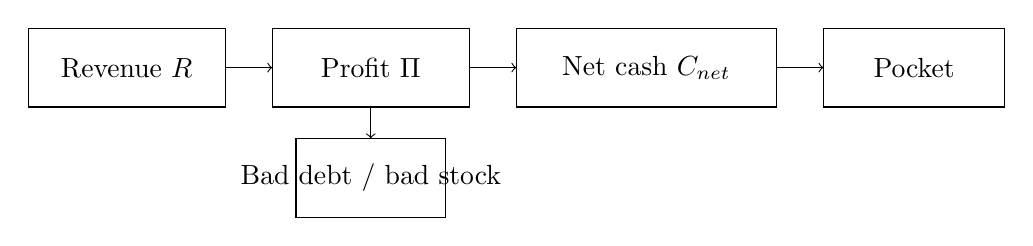
\begin{tikzpicture}[x=1cm,y=1cm]
\draw (0,0) rectangle (2.5,1) node[pos=.5] {Revenue $R$};
\draw (3.1,0) rectangle (5.6,1) node[pos=.5] {Profit $\Pi$};
\draw (6.2,0) rectangle (9.5,1) node[pos=.5] {Net cash $C_{\text{net}}$};
\draw (10.1,0) rectangle (12.4,1) node[pos=.5] {Pocket};
\draw[->] (2.5,.5) -- (3.1,.5);
\draw[->] (5.6,.5) -- (6.2,.5);
\draw[->] (9.5,.5) -- (10.1,.5);
\draw (3.4,-1.4) rectangle (5.3,-.4) node[pos=.5] {Bad debt / bad stock};
\draw[->] (4.35,0) -- (4.35,-.4);
\end{tikzpicture}
\end{figure}

The diagram is a transcript-backed reconstruction rather than a transcription of any visible board. Its purpose is only to keep the lecture's ranking of quantities in view. We begin with top-line magnitude, pass through the accounting mask, and end with the only number the interview is willing to honor without qualification: extractable cash.

\begin{remark}
The interview gives a ranking, not a full accounting identity. The notation \(R\), \(\Pi\), and \(C_{\text{net}}\) is therefore a careful reconstruction of the spoken distinction, not a claim about the lecturer's exact symbols.
\end{remark}

\section{Mentors, Mobility, and the Poverty Loop}

Once the cash question is settled, the lecture widens again. This widening matters. We are not allowed to leave the discussion as though wealth were merely an accounting puzzle. The first billionaire now turns outward and describes wealth as a social and geographical process.

The lecture's strongest social claim is that poverty is escaped by attaching oneself to different examples. One should, she says, become friends with at least one rich person, because the rich will teach, mentor, introduce, and sometimes even fund. The statement is severe and deliberately provocative. Still, its mechanism is clear enough. The poor and the rich do not merely hold different quantities of capital. They inhabit different circles of imitation.

At this point the lecturer briefly steps back and recaps the interview in plain language. What keeps poor people poor, he says, is that they do not attach themselves to the right people. This recap should be preserved, because it shows the lecture doing what it repeatedly does: compressing testimony into a portable rule before moving on.

The same movement from biography to mechanism appears again in the travel advice. Leaving one's hometown is not treated here as cosmetic sophistication. It is treated as a change in coordinates. One crosses the ocean, exits comfort, and is forced into a different set of perceptions. In the interview's own language, one's neurons change.

\subsection{Question \& Answer}

Can we become rich while staying comfortable, local, and approved?

The lecture's answer is no, or at least not by the path it is describing. Approval seeking wastes energy. Staying fixed preserves the size of the world one already inhabits. Movement creates exposure, and exposure changes ambition, judgment, and opportunity.

We may summarize the lecture's logic schematically as
\begin{equation}
\text{movement} \to \text{discomfort} \to \text{exposure} \to \text{change of self and business horizon}.
\end{equation}
The line ``you're not a tree'' is playful, but it carries the whole idea. Human capital is mobile. If one insists on sitting on a couch, then at least that couch should be in Paris. The lecture is not praising tourism as such. It is attacking the economics of fixed identity.

The closing line of this stretch pushes the same thought one level deeper. Things happen for you, not merely to you. Adversity is not denied. It is reclassified. Difficulty becomes preparation. In that sense the lecture is still talking about the same initial condition \(D_0<0\), only now in psychological form. The hole from which one begins need not determine the horizon one later sees.

\section{Communication as Economic Infrastructure}

The next interview turns the lecture sharply from portfolio wealth to communication wealth. The transition is not arbitrary. The first billionaire has just said that who we attach ourselves to matters. The next subject, Dr. Forbes Riley, now insists that how we reach people matters just as much.

The interview begins, again, with scale. She says she created one of the great fitness products on the planet, but immediately refuses to be described merely as a business owner. She also, she says, masters the art of communication. The lecture then condenses that claim into monetary scale:
\begin{align}
V_{\text{sales}} &> \$2.5 \times 10^9,\\
R_{\text{day}} &= \$1 \times 10^6/\text{day}.
\end{align}
These are sales claims, not claims about net worth or profit. The distinction matters, and the lecture is increasingly careful about such distinctions.

The conceptual core of the segment is unusually clean. Pitching is defined not rhetorically but operationally. It is the art of getting someone to say yes. That first yes matters because it opens the next gate: a credit card, a meeting, an order, a channel, representation, a chance. The lecture is therefore treating communication as leverage, not ornament.

A cautious formal summary is
\begin{equation}
\text{communication} \to \text{persuasion} \to \text{yes} \to \text{access/opportunity}.
\end{equation}
Nothing more elaborate is required. The lecture's point is not algebraic. It is structural. If one can reliably produce the next yes, one can repeatedly convert speech into leverage.

The event interruption strengthens rather than weakens the argument. Filming must pause. Privacy asserts itself. The setting resists documentation. Dr. Forbes Riley answers by giving the rule ``don't ask for permission; ask for forgiveness,'' and then justifies it with a concrete story. Unable to secure an agent, she created a manager, created a company, and represented herself. The institutional gate was closed, so she manufactured the missing institution.

Here too the lecture recaps. After the first two entrepreneurial interviews, the lecturer stops and states one common principle: they mastered attention. The long interlude on content and audience growth may be compressed heavily, but one structural point should remain. In the lecture's world, attention is not a vanity metric. It is convertible leverage.

\section{Attention, Athletics, and Preservation}

The Miles Garrett interview asks whether these earlier rules persist once wealth no longer comes from selling a product but from elite athletic performance. The lecture's answer is yes, though the emphasis shifts from selling to preserving.

The interviewer first fixes scale by climbing a ladder of thresholds, each of which Garrett clears. The transcript therefore supports a lower bound rather than an exact annual figure:
\begin{equation}
Y_{\text{Miles}} > \$20 \times 10^6.
\end{equation}

\paragraph{A clean lower bound.}
It is worth writing the derivation plainly.
\begin{enumerate}
\item The interviewer asks whether the annual amount exceeds \$10 million.
\item Garrett says yes.
\item The threshold is raised to \$15 million.
\item Garrett again says yes.
\item The threshold is raised once more to \$20 million.
\item Garrett again says yes.
\item Therefore the transcript warrants a lower bound, not a point estimate: \(Y_{\text{Miles}} > \$20 \times 10^6\).
\end{enumerate}

Once again the lecture reverses from scale to origin. Garrett did not come from money. His motivation is familial, especially his grandmother, whose memory remains attached to his work. The interview then asks the natural follow-up: not how to make money, but how to keep it from evaporating.

His answer is brief but concrete. He names teams and renewable energy, then adds part ownership in the Cavaliers and a desire for ownership in a Premier League club. The lecture does not give us weights or portfolio percentages, and we should not invent them. But the direction is plain enough. Current earnings are to be converted into durable claims on future enterprises.

The deepest line of the section, however, is not financial vocabulary at all. In high school, he was told to be all in or all out. That sentence functions in the lecture almost as a rule of motion:
\begin{equation}
\text{elite outcome} \Longrightarrow \text{total commitment}.
\end{equation}
We need not pretend this is a numerical law. It is a disciplined verbal one. If the desired output is greatness, then half-participation is excluded by definition.

The section closes by returning to motive and order. Garrett says he does not worry about haters. He gives glory to God. The lecturer's recap after the interview reduces the whole segment to two lines: all in or all out, and all glory to God. That recap should remain, because it shows how the lecture itself chooses to compress athletic wealth into an ethic of total commitment under faith.

\section{Spend, Trust, and the Arithmetic of Enough}

The final movement changes both setting and code. We leave the street and go to the Beverly Hills Hilton for the Legend of Aviation Awards. The interviewer explicitly changes out of casual streetwear and into a suit because access now runs not only through persistence but through costume. This detail should stay. The lecture is showing that entry conditions themselves vary by social layer.

Inside, the interview with Ken Richie of Flexjet gives us the cleanest quantitative heuristic in the chapter. First, though, the lecture again secures company scale:
\begin{align}
N_{\text{planes}} &\approx 370,\\
N_{\text{employees}} &\approx 5000.
\end{align}
Only after this does the interview move to the more general trait inventory: passion, and then fanatical attention to detail. Large outcomes, the lecture suggests, are not only driven by large desires. They are stabilized by care for small asymmetries.

\subsection{Question \& Answer}

When are we actually rich?

This is the lecture's cleanest explicit financial question, and the answer is given with a formula.

\begin{definition}
Let \(S\) denote annual spend, the amount required to live the life one actually wishes to live. The interview's heuristic threshold for being rich is
\begin{equation}
W^\ast = 25S,
\end{equation}
where \(W^\ast\) is the wealth stock sufficient to support that spend at the lecture's chosen multiple.
\end{definition}

The lecturer immediately supplies examples, and we should preserve them because they show how the rule is meant to work:
\begin{align}
S &= \$1000/\text{year}
\qquad \Longrightarrow \qquad
W^\ast = \$25{,}000,\\
S &= \$10 \times 10^6/\text{year}
\qquad \Longrightarrow \qquad
W^\ast = \$250 \times 10^6.
\end{align}
The point is corrective. ``Ten million'' and ``twelve million'' are treated as the wrong style of question. The right question is lifestyle-relative: what does it actually cost to live the life one intends to live? Wealth is thus tied to burn rate rather than to social theater.

\begin{remark}
The factor \(25\) is presented in the interview as a rule of thumb rather than as a universal theorem of finance. The notes should preserve it with exactly that status.
\end{remark}

The lecture could have ended there, with enough as arithmetic, but it does not. It turns instead to family money culture and trust. Ken says that households have learned to speak more freely about sex than about money, even though money is one of the central practical realities children must eventually steward. He then recounts advice from President Clinton: trust is created when one discloses a fault. The extension to family life is immediate. If one wants children to trust parents around money, then money cannot remain one of the untouchable family secrets.

The final question completes the chapter's arc. Asked what single message he would leave to the younger generation, Ken answers with empathy. Think about others, employees, family, and the way people remember how one made them feel. The lecture begins from billionaires and ends from human memory. Arithmetic remains on the page, but it no longer stands alone.

\section{Summary}

This lecture unfolds by moving from spectacle to mechanism. First, wealth is shown in public. Then it is broken into transferable parts. From the first billionaire we get the chapter's strictest business distinction: not revenue, not even nominal profit, but after-tax cash that can really be extracted from the business. From the next segment we learn that communication is not decoration but leverage, because the first yes can open all the later gates. From Miles Garrett we see that high income is only the beginning; preservation, total commitment, and motive must follow. And from Ken Richie we get the chapter's clearest arithmetic: if annual spend is \(S\), then the lecture's threshold for being rich is \(W^\ast = 25S\). The final turn is the most instructive of all. Wealth is not left as a pile of numbers. It is joined to stewardship, disclosure, trust, and empathy.